\documentclass[12pt, a4paper, twoside]{article}

%% Preamble
\usepackage{umatfgspanish}
\graphicspath{{./images/}}

\begin{document}

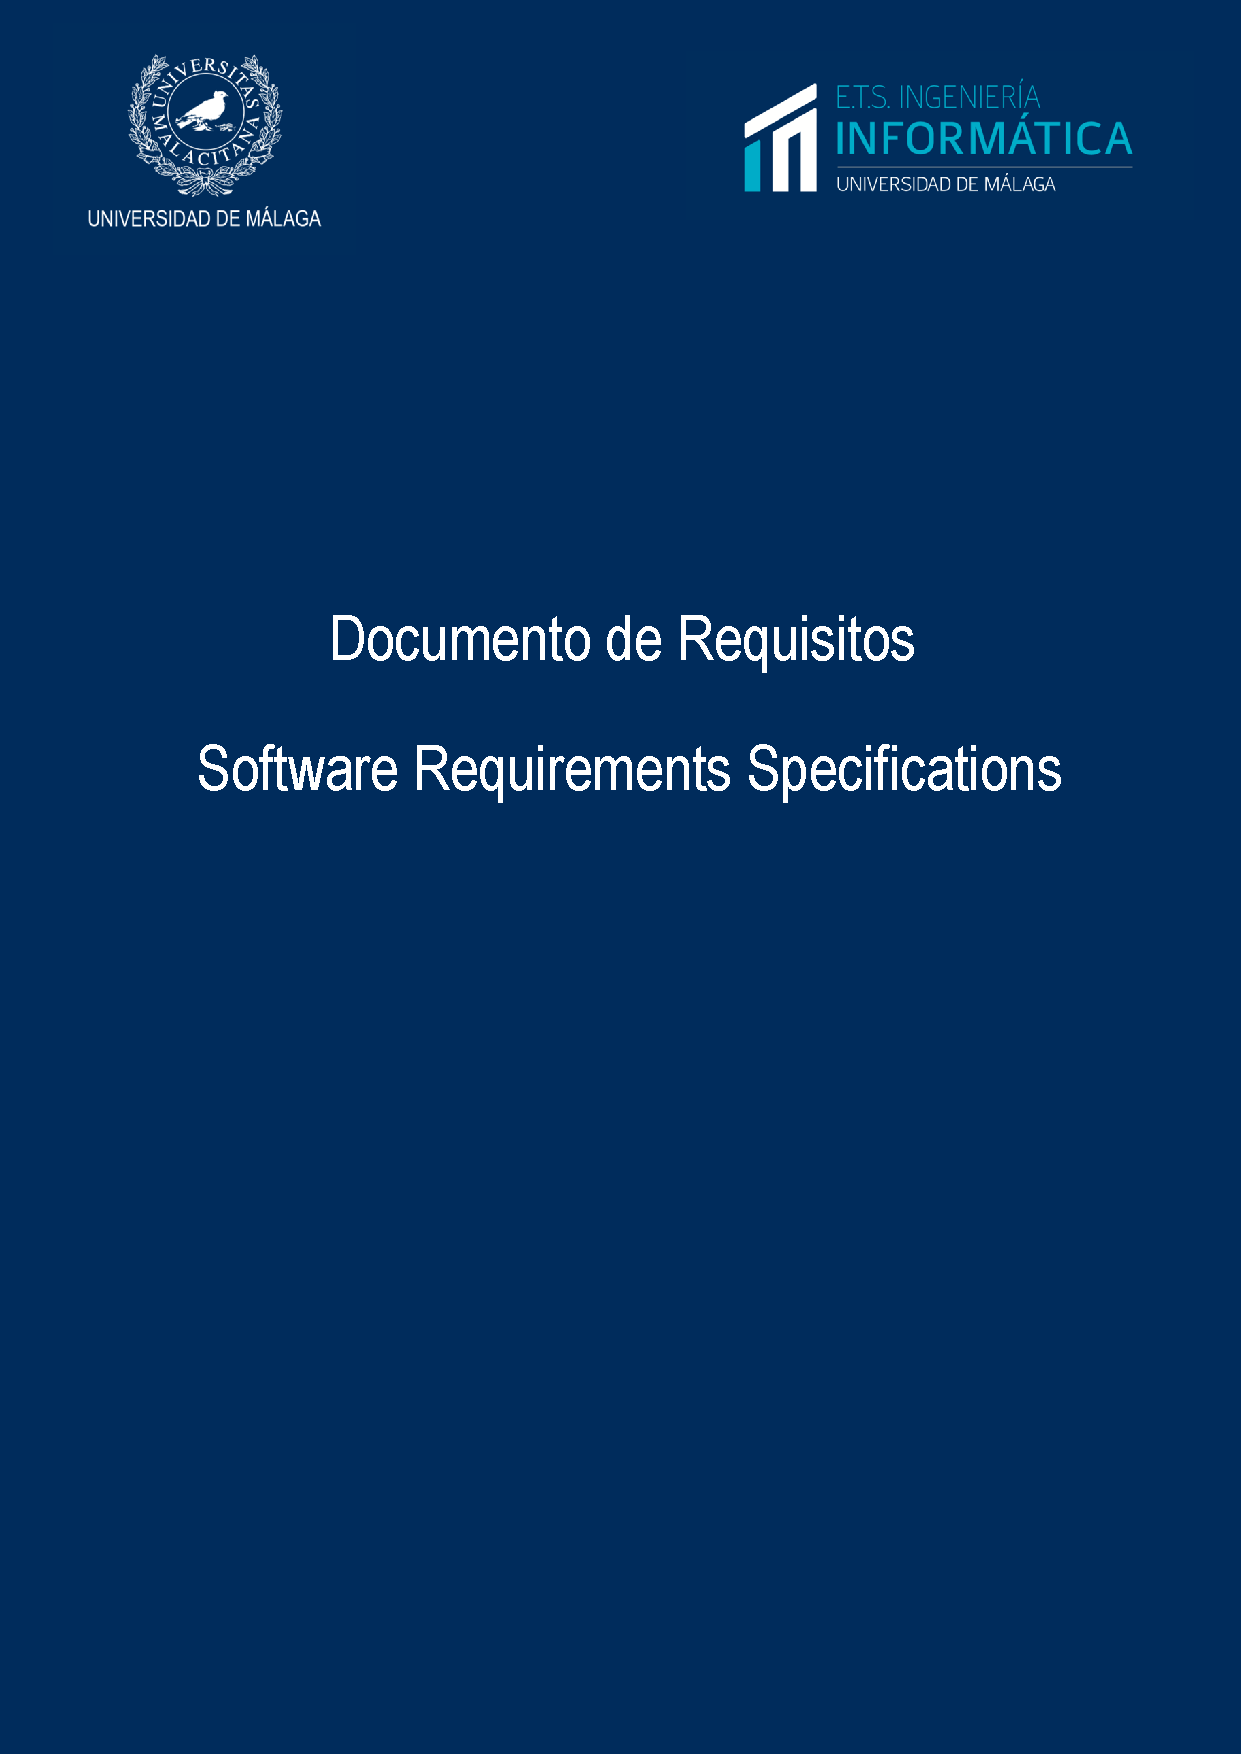
\includepdf[noautoscale=true, width=\paperwidth]{title.pdf}

\newpage

\tableofcontents

%% Sections
\section{Síntesis del documento}
\section{Propósito}
\subsection{Propósito}
Desarrollar un Software que permita interactuar con cualquier elemento 
integrable a la red de Internet que se encuentre en un edificio.
\section{Proceso de Análisis del Negocio}
\section{Ámbito}
Debido a las características del software que hacen uso de las tecnologías 
\"Internet de las Cosas\" (IoT) para la gestión de dispositivos conectados a
la red de un Edificio Inteligente (Smart Building), se ha decidido darle el nombre de
\"IoTBuildingManagement\".

IoTBuildingManagement será el módulo principal al que se podrán conectar diversos pluggins para la
gestión de dispositivos IoT concretos dentro de un edificio. Cada pluggin deberá de tener 
la lógica para controlar los datos de un dispositivo específico.

IoTBuildingManagement deberá tener la lógica necesaria para que los dispositivos IoT
puedan coordinarse entre sí.

\subsection{Preparación para el Análisis del Negocio}
\subsubsection{Contextualización}
El contexto que se va a desarrollar a continuación parte del concepto de Internet de las Cosas (IoT).

Internet consiste en una red de usuarios y servidores conectadas entre sí.
Sin embargo, existen conceptos más amplios que abarcan un conjunto de elementos todavía más ambicioso,
como es el de IoT, que, además de los anteriores, incluye a cualquier objeto físico como participante de la red.

De esta forma podemos ser capaces de interactuar con los objetos de manera remota, sin intervención física de
una persona, o de manera automática.

Además, podrían realizar sus tareas de forma más inteligente, ya que, al estar conectadas a internet, pueden
disponer de mucha información útil para su objetivo.

Desde que se empezó a aplicar el concepto de IoT, se puede ver que ha ocurrido una evolución y ha mejorando en
muchos los aspectos: El presupuesto invertido en la IoT ha incrementado, el número de dispositivos ha crecido
exponencialmente, ...

También es destacable mencionar que la situación global de la COVID-19 ha incentivado y acelerado la aplicación
de la IoT en diversos aspectos como la salud pública, la seguridad o la privacidad.
(
En los últimos años, el uso del IoT ha aumentado exponencialmente [ENSEÑAME LO QUE TIENES].
Elnashar, A. \& El-saidny, M. (2018). IoT evolution towards a super-connected world. Wiley. \textit{Practical Guide to LTE-A, VoLTE and IoT: Paving the way towards 5G}. pp. 310-381. Wiley. https://doi.org/10.1002/9781119063407.ch7
Ayman Elnashar; Mohamed A. El-saidny, "IoT Evolution Towards a Super‐connected World," in Practical Guide to LTE-A, VoLTE and IoT: Paving the way towards 5G , Wiley, 2018, pp.310-381, doi: 10.1002/9781119063407.ch7.




)
\subsubsection{Problemas y oportunidades identificadas}
REF: 
Estevez E., Pardo, T., \& Scholl, J. (2021). Smart cities and smart governance: towards the 22nd century sustainable city. Springer.

La IoT es una tecnología relativamente reciente y son muchos los campos los que se pueden beneficiar de su uso:
ciudades inteligentes, agricultura, Smart Home, 
Una oportunidad identificada es el hecho de que el IoT es una tecnología muy reciente y todavía
no se ha aplicado en numerosos campos 

Se puede identificar una oportunidad en el hecho de que hay muchos campos de aplicación en los que se
puede aplicar el IoT y todavía no se ha hecho uso de.
El IoT es una tecnología que lleva poco tiempo en auge y son muchos los campos en los que se puede 
aplicar para sacar ventaja, obtener beneficios, mejorar la calidad...

Se puede identificar un problema en [LAS COSAS ESTAS DE CIUDADES]

El potencial que se le puede sacar a esta red de dispositivos es muy elevado. Existen conceptos tales como:
 - IoT Orchestation
 - Fog Computing
 - 
\end{document}